\section{静电学问题}
\subsection{立方电阻网}
\subsubsection{有限立方电阻网}
在 \(d\) 个相互独立的方向上，组成 \(N_1 \times N_2 \times \cdots \times N_d\) 的立方电阻网，第 \(q\) 个方向（\(q = 1, \ldots, d\)）由 \(N_q\) 个阻值均为 \(a_q r\) 的电阻连接而成，\(d\) 个方向相互交叉形成 \(\prod_q N_q\) 个连接点。选取电阻网角落连接点为原点，求 \((x_1, \ldots, x_d)\) 与 \((y_1, \ldots, y_d)\) 两连接点之间的电阻。

对 \(d\) 个方向进行对称化及周期化操作（即如图\ref{立方电阻网对称化示意图}），由于原问题电流无法从边界流出，故操作后边界条件仍然满足，原区域的解就是原问题的解。
\begin{figure}[htbp]
	\centering
	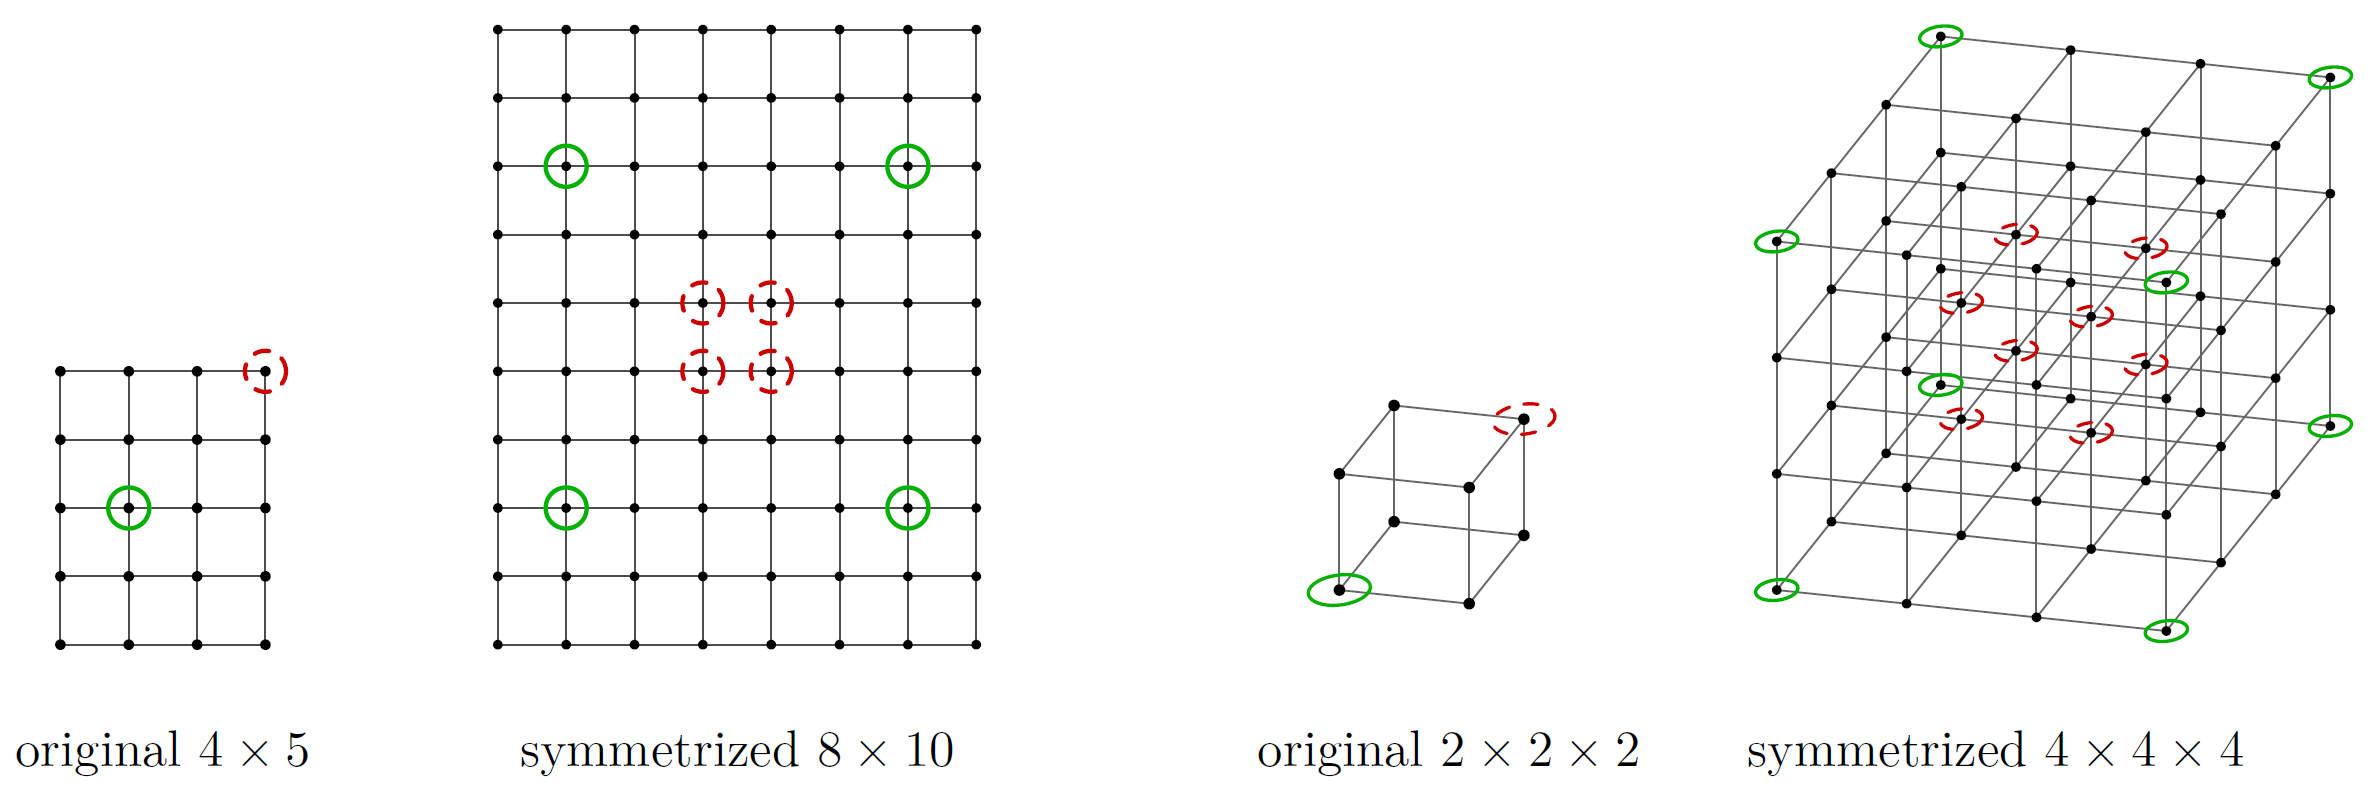
\includegraphics[width=0.8\textwidth]{electrostatics_fig/cubic_resistor_network_symmetrization_schematic_diagram.png}
	\caption{立方电阻网对称化示意图}
	\label{立方电阻网对称化示意图}
\end{figure}

操作后，重新规定坐标零点，则电流的注入和注出点（各 \(2^d\) 个）为：
\begin{equation*}
	r_{\text{in}} = (x_1, x_2, \ldots, x_d),\ (2N_1 - x_1 - 1, x_2, \ldots, x_d),\ \ldots,\ (2N_1 - x_1 - 1, 2N_2 - x_2 - 1, \ldots, 2N_d - x_d - 1).
\end{equation*}
\begin{equation*}
	r_{\text{out}} = (y_1, y_2, \ldots, y_d),\ (2N_1 - y_1 - 1, y_2, \ldots, y_d),\ \ldots,\ (2N_1 - y_1 - 1, 2N_2 - y_2 - 1, \ldots, 2N_d - y_d - 1).
\end{equation*}

记注入电流为 \(I\)，连接点 \((\xi_1, \ldots, \xi_d)\) 的注入电流为 \(I\,[\xi_1, \ldots, \xi_d]\)，连接点 \((\xi_1, \ldots, \xi_d)\) 的电压为 \(U\,[\xi_1, \ldots, \xi_d]\)，则电路方程为
\begin{equation*}
	&\sum_q \dfrac{1}{2a_q} \left( 2U[\xi_1, \ldots, \xi_d] - U[\xi_1, \ldots, \xi_q - 1, \ldots, \xi_d] - U[\xi_1, \ldots, \xi_q + 1, \ldots, \xi_d] \right) = rI[\xi_1, \ldots, \xi_d].\\
	&I[\xi_1, \ldots, \xi_d] =
	\begin{cases}
		I,  & [\xi_1, \ldots, \xi_d] = r_{\text{in}}  \\
		-I, & [\xi_1, \ldots, \xi_d] = r_{\text{out}} \\
		0,  & \text{else}
	\end{cases}.
\end{equation*}

操作后问题具有周期性，\(\xi_q\) 以 \(2N_q - 1\) 为周期，可以对 \(U\) 和 \(I\) 做离散傅里叶变换：
\begin{equation*}
	&U[\xi_1, \ldots, \xi_d] = \dfrac{1}{2^d \prod_q N_q} \prod_q \sum_{k_q} A[k_1, \ldots, k_d] \exp\left( i\pi \sum_q \dfrac{k_q \xi_q}{N_q} \right).\\
	&A[k_1, \ldots, k_d] = \prod_q \sum_{\xi_q} U[\xi_1, \ldots, \xi_d] \exp\left( -i\pi \sum_q \dfrac{k_q \xi_q}{N_q} \right).\\
	&k_q,\,\xi_q = 0, 1, \ldots, 2N_q - 1,\quad\prod_q \sum_{\xi_q} = \sum_{\xi_1} \cdots \sum_{\xi_d}
\end{equation*}
得：
\small
\begin{align*}
	 & \qquad\sum_q \dfrac{2}{a_q} \left( 1 - \cos\left( \dfrac{\pi k_q}{N_q} \right) \right) A[k_1, \ldots, k_d]                                                                                                                                                               \\
	 & = rI \Bigg[ \prod_q \left( \exp\left( -i\pi \sum_q \dfrac{k_q x_q}{N_q} \right) + \exp\left( -i\pi \sum_q \dfrac{k_q (2N_q - x_q - 1)}{N_q} \right) \right)                                                                                                              \\
	 & \qquad -\prod_q \left( \exp\left( -i\pi \sum_q \dfrac{k_q y_q}{N_q} \right) + \exp\left( -i\pi \sum_q \dfrac{k_q (2N_q - y_q - 1)}{N_q} \right) \right)
	\Bigg]                                                                                                                                                                                                                                                                      \\
	 & = 2^d rI \exp\left( -i \sum_q \dfrac{\pi k_q (2N_q - 1)}{2N_q} \right) \Bigg( \prod_q \cos\left( \dfrac{k_q \left( x_q - \dfrac{2N_q - 1}{2} \right) \pi}{N_q} \right) - \prod_q \cos\left( \dfrac{k_q \left( y_q - \dfrac{2N_q - 1}{2} \right) \pi}{N_q} \right) \Bigg) \\
	 & = 2^d rI \exp\left( i \sum_q \dfrac{\pi k_q}{2N_q} \right) \Bigg[ \prod_q \cos\left( \dfrac{k_q \left( x_q + \dfrac{1}{2} \right) \pi}{N_q} \right) - \prod_q \cos\left( \dfrac{k_q \left( y_q + \dfrac{1}{2} \right) \pi}{N_q} \right) \Bigg]
\end{align*}
\normalsize
也即
\begin{equation*}
	A\,[k_1, \ldots, k_d] = \dfrac{2^{d-1} rI}{\sum_q \dfrac{1}{a_q} \left( 1 - \cos\left( \dfrac{\pi k_q}{N_q} \right) \right)} \exp\left( i \sum_q \dfrac{\pi k_q}{2N_q} \right) \left( \prod_q \cos\left( \dfrac{k_q (x_q + \dfrac{1}{2}) \pi}{N_q} \right) - \prod_q \cos\left( \dfrac{k_q (y_q + \dfrac{1}{2}) \pi}{N_q} \right) \right).
\end{equation*}
进而，\((x_1, \ldots, x_d)\) 与 \((y_1, \ldots, y_d)\) 两连接点之间的电阻为：
\small
\begin{align*}
	R & = \dfrac{1}{I} \left( U[x_1, \ldots, x_d] - U[y_1, \ldots, y_d] \right)                                                                                                                                                                                                                                \\
	  & = \dfrac{r}{2^d \prod_q N_q} \prod_q \sum_{k_q} A[k_1, \ldots, k_d] \left( \exp\left( i\pi \sum_q \dfrac{k_q x_q}{N_q} \right) - \exp\left( i\pi \sum_q \dfrac{k_q y_q}{N_q} \right) \right)                                                                                                           \\
	  & = \dfrac{r}{2 \prod_q N_q} \prod_q \sum_{k_q} \dfrac{1}{\sum_q \dfrac{1}{a_q} \left( 1 - \cos\left( \dfrac{\pi k_q}{N_q} \right) \right)} \left[ \prod_q \cos\left( \dfrac{k_q (x_q + \dfrac{1}{2}) \pi}{N_q} \right) - \prod_q \cos\left( \dfrac{k_q (y_q + \dfrac{1}{2}) \pi}{N_q} \right) \right]^2
\end{align*}

\normalsize
\begin{example}
	对于一个各项同性的二维电阻网\(d = 2,\,a_1 = a_2 = 1.\)
	\small
	\begin{equation*}
		R = \dfrac{r}{2 N_1 N_2} \sum_{k_1=0}^{2N_1 - 1}\, \sum_{k_2=0}^{2N_2 - 1} \dfrac{\left[\, \cos\left( \dfrac{\pi k_1 (x_1 + \dfrac{1}{2})}{N_1} \right) \cos\left( \dfrac{\pi k_2 (x_2 + \dfrac{1}{2})}{N_2} \right) - \cos\left( \dfrac{\pi k_1 (y_1 + \dfrac{1}{2})}{N_1} \right) \cos\left( \dfrac{\pi k_2 (y_2 + \dfrac{1}{2})}{N_2} \right) \,\right]^2}{2 - \cos\left( \dfrac{\pi k_1}{N_1} \right) - \cos\left( \dfrac{\pi k_2}{N_2} \right)}.
	\end{equation*}

	\normalsize
	比如，对于结构\(N_1 = N\)，\(N_2 = 2\)，\((x_1, x_2) = (x, 2)\)，\((y_1, y_2) = (y, 1)\) 可以解析求得
	\begin{align*}
		R  & = \dfrac{r}{4 N} \sum_{k_1=0}^{2N - 1} \sum_{k_2=0}^{3}
		\dfrac{\left[\,
				\cos\left( \dfrac{\pi k_1 (x + \dfrac{1}{2})}{N} \right)
				\cos\left( \dfrac{3 \pi k_2}{4} \right)
				-
				\cos\left( \dfrac{\pi k_1 (y + \dfrac{1}{2})}{N} \right)
				\cos\left( \dfrac{\pi k_2}{4} \right) \,
				\right]^2}
		{2 - \cos\left( \dfrac{\pi k_1}{N} \right) - \cos\left( \dfrac{\pi k_2}{2} \right)}                                               \\[1em]
		   & = \dfrac{r}{2} \left| x - y \right| +
		\dfrac{r}{4 \sqrt{3} \left( 1 - \beta^{2N} \right)} \Bigg(
		\beta^{2N - 1 - 2x} + \beta^{2N - 1 - 2y} + \beta^{2x + 1} + \beta^{2y + 1}                                                       \\ &\qquad+2\beta^{2N - 1 - x - y} + 2\beta^{x + y + 1} + 2 + 2\beta^{2N} + 2\beta^{\left| x - y \right|} + 2\beta^{2N - \left| x - y \right|}
		\Bigg).                                                                                                                           \\
		R| & _{1 \ll x, y \ll N} = \dfrac{r}{2} \left( |x - y| + \dfrac{\sqrt{3}}{3} \left( 1 + (2 - \sqrt{3})^{|x - y|} \right) \right).
	\end{align*}
	式中 \(\beta = 2 - \sqrt{3}\)。
\end{example}

\subsubsection{无限立方电阻网}
在 \(d\) 个相互独立的方向上，组成无限延伸的立方电阻网，第 \(q\) 个方向（\(q = 1, \ldots, d\)）由无限多阻值均为 \(a_q r\) 的电阻连接而成，\(d\) 个方向相互交叉形成无数个连接点。选取电阻网内任意连接点为原点，求它与 \((x_1, \ldots, x_d)\) 连接点之间的电阻。

记注入电流为 \(I\)，连接点 \((\xi_1, \ldots, \xi_d)\) 的注入电流为 \(I\,[\xi_1, \ldots, \xi_d]\)，连接点 \((\xi_1, \ldots, \xi_d)\) 的电压为 \(U\,[\xi_1, \ldots, \xi_d]\)，进而给出电路方程为
\begin{equation*}
	&\sum_q \dfrac{1}{2a_q} \left( 2U[\xi_1, \ldots, \xi_d] - U[\xi_1, \ldots, \xi_q - 1, \ldots, \xi_d] - U[\xi_1, \ldots, \xi_q + 1, \ldots, \xi_d] \right) = rI[\xi_1, \ldots, \xi_d].\\
	&I[\xi_1, \ldots, \xi_d] =
	\begin{cases}
		I,  & [\xi_1, \ldots, \xi_d] = [0, \ldots, 0]     \\
		-I, & [\xi_1, \ldots, \xi_d] = [x_1, \ldots, x_d] \\
		0,  & \text{else}
	\end{cases}.
\end{equation*}

\(\xi_q\) 从 \(-\infty\) 到 \(+\infty\) 取离散整数值，可以对 \(U\) 和 \(I\) 做无限傅里叶变换：
\begin{equation*}
	&U[\xi_1, \ldots, \xi_d] = \dfrac{1}{(2\pi)^d} \prod_q \int_{-\pi}^{\pi} A(k_1, \ldots, k_d) \exp\left( i \sum_q k_q \xi_q \right) \prod_q \d k_q.\\
	&A(k_1, \ldots, k_d) = \prod_q \sum_{\xi_q} U[\xi_1, \ldots, \xi_d] \exp\left( -i \sum_q k_q \xi_q \right).
\end{equation*}
其中 \(k_q\) 从 \(-\infty\) 到 \(+\infty\) 连续取值，\(\prod_q \sum_{\xi_q} = \sum_{\xi_1} \cdots \sum_{\xi_d}\)，\(\prod_q \int_{-\pi}^{\pi} = \int_{-\pi}^{\pi} \cdots \int_{-\pi}^{\pi}\)（对 \(d\) 个变量积分）。

回代回路方程得：
\begin{equation*}
	\sum_q \dfrac{2}{a_q} (1 - \cos k_q) A(k_1, \ldots, k_d) = rI \left( 1 - \exp\left( -i \sum_q k_q x_q \right) \right).
\end{equation*}
即
\begin{equation*}
	&A(k_1, \ldots, k_d) = \dfrac{rI \left( 1 - \exp\left( -i \sum_q k_q x_q \right) \right)}{\sum_q \dfrac{2}{a_q} (1 - \cos k_q)}.\\
	&U[\xi_1, \ldots, \xi_d] = \dfrac{1}{(2\pi)^d} \prod_q\int_{-\pi}^{\pi} rI \cdot \dfrac{1 - \exp\left( -i \sum_q k_q x_q \right)}{\sum_q \dfrac{2}{a_q} (1 - \cos k_q)} \exp\left( i \sum_q k_q \xi_q \right) \prod_q dk_q.
\end{equation*}

原点与 \((x_1, \ldots, x_d)\) 之间的电阻为：
\begin{equation*}
	R(x_1, \ldots, x_d) = \dfrac{1}{I} \left( U[x_1, \ldots, x_d] - U[0, \ldots, 0] \right) = \dfrac{r}{(2\pi)^d} \prod_q \int_{-\pi}^{\pi} \dfrac{1 - \cos\left( \sum_q k_q x_q \right)}{\sum_q \dfrac{1}{a_q} (1 - \cos k_q)} \prod_q dk_q.
\end{equation*}

\begin{example}
	对于各项同性的二维无限电阻网
	\begin{equation*}
		d = 2, \quad a_1 = a_2 = 1.
	\end{equation*}
	\begin{equation*}
		R(x_1, x_2) = \dfrac{r}{4\pi^2} \int_{-\pi}^{\pi} \int_{-\pi}^{\pi} \dfrac{1 - \cos\left( k_1 x_1 + k_2 x_2 \right)}{2 - \cos k_1 - \cos k_2} dk_1 dk_2.
	\end{equation*}
	不难算得：
	\begin{equation*}
		R(1, 0) = \dfrac{1}{2} r, \quad R(1, 1) = \dfrac{2}{\pi} r, \quad R(1, 2) = \left( \dfrac{4}{\pi} - \dfrac{1}{2} \right) r, \quad R(2, 0) = \left( 2 - \dfrac{4}{\pi} \right) r,
	\end{equation*}
	\begin{equation*}
		\quad R(3, 0) = \left( \dfrac{17}{2} - \dfrac{24}{\pi} \right) r, \quad R(1, 3) = 2.7670 r, \quad R(2, 3) = 2.9041 r.
	\end{equation*}
\end{example}

\subsection{椭球的静电性质}
\subsubsection{导体椭球的电容}
记椭球的三个轴的半长为  \(a, b, c (a\geq b \geq c)\)，选取椭球坐标\(\xi,\,\eta,\,\zeta\)，相关数学公式见\ref{椭球坐标系小节}.令椭球带电量为\(Q\)，考虑到椭球表面 (对应\(\xi = 0\)) 是等势面，猜测空间电势分布只与\(\xi\)有关，即：
\begin{equation*}
	\Phi(\xi,\eta,\zeta)=\Phi(\xi),
	\qquad
	\nabla^2\Phi(\xi)
	=\frac{4\sqrt{\varphi(\xi)}}{(\xi-\eta)(\xi-\zeta)}
	\frac{\d}{\d \xi}\Bigl(\sqrt{\varphi(\xi)}\,
	\frac{\d \Phi}{\d \xi}\Bigr)
	=0,
	\quad
	\Phi(\xi\to\infty)=0,
\end{equation*}
其中
\(\displaystyle
\varphi(\Theta)=(a^2+\Theta)(b^2+\Theta)(c^2+\Theta).
\)

求解微分方程，得到电势、电场、表面电荷密度为：
\begin{equation*}
	\Phi(\xi)
	&=A \int_{\xi}^{\infty}\frac{\d \Theta}{\sqrt{\varphi(\Theta)}},\quad
	\vb{E}
	=-\nabla\Phi
	=-\frac{\d \Phi/\d \xi}{h_{\xi}}\,
	\uv{e}_{\xi}
	=\frac{2A}{\sqrt{(\xi-\eta)(\xi-\zeta)}}\,
	\uv{e}_{\xi}.\\
	\sigma
	&=\varepsilon_{0}\,\uv{e}_{\xi}\!\cdot\vb{E}\big|_{\xi=0}
	=\frac{2\varepsilon_{0}A}{\sqrt{\eta\,\zeta}}
	=\frac{2\varepsilon_{0}A}{a\,b\,c}\,\left( \frac{x^2}{a^4} + \frac{y^2}{b^4} + \frac{z^2}{c^4} \right)^{-1/2}.
\end{equation*}

根据总电荷归一化条件，得到待定常数\(A\)如下
\begin{equation*}
	Q=\iint_{\xi=0}\sigma\,\d S
	\quad\Longrightarrow\quad
	A=\frac{Q}{8\pi\varepsilon_{0}}.
\end{equation*}

回代得最终结果为
\begin{equation*}
	&\Phi(\xi)
	=\frac{Q}{8\pi\varepsilon_{0}}\;\Lambda(\xi),\quad
	\vb{E}
	=\frac{Q}{4\pi\varepsilon_{0}\,\sqrt{(\xi-\eta)(\xi-\zeta)}}\,
	\uv{e}_{\xi},\quad
	\sigma
	=\frac{Q}{4\pi\,a b c}\,
	\left( \frac{x^2}{a^4} + \frac{y^2}{b^4} + \frac{z^2}{c^4} \right)^{-1/2}\\
	&C_{\mathrm{ellipsoid}}
	=\frac{Q}{\Phi(0)}
	=\frac{8\pi\varepsilon_{0}}{\Lambda(0)}=\frac{4\pi\varepsilon_{0} \sqrt{a^2 - b^2} }{F\left( \sqrt{ \dfrac{a^2 - c^2}{a^2 - b^2} },\,
		\arcsin \sqrt{ \dfrac{a^2 - b^2}{a^2} } \right)}
\end{equation*}

在远处，带电椭球的最低阶非零阶电场效应为电四极矩：
\begin{equation*}
	\vb{D} = \int_S \left(3\,\vb{r}\,\vb{r} - r^2\, \vb{I}\,\right) \sigma \, \d S
	= \frac{Q}{3} \left[
		(2a^2 - b^2 - c^2) \uv{x}\,\uv{x}\, +
		(2b^2 - c^2 - a^2) \uv{y}\,\uv{y}\, +
		(2c^2 - a^2 - b^2) \uv{z}\,\uv{z}\,
		\right]
\end{equation*}
\subsubsection{介质椭球在匀强电场中的极化}

在介电常数为 \(\varepsilon_1\) 的无限大空间中，有介电常数为 \(\varepsilon_2\) 的椭球体，三个轴的半长为 \(a\ge b\ge c\)，沿其轴建立直角坐标系 \(x\)–\(y\)–\(z\)，原点在椭球中心.在空间中施加外电场 \(\vb{E}_0\)，介质椭球产生极化，形成新的空间电势.

引入椭球坐标系 \(\xi\)–\(\eta\)–\(\zeta\)，其与直角坐标系的转换关系如前所述.

先考虑外电场 \(x\) 分量 \(E_{0x}\) 的影响，记无椭球时其产生的电势分布为
\begin{equation*}
	f_x(\xi,\eta,\zeta)=-E_{0x}\,x
	=\pm E_{0x}\sqrt{\frac{(a^2+\xi)(a^2+\eta)(a^2+\zeta)}{(a^2-b^2)(a^2-c^2)}},
\end{equation*}
\(x<0\) 取上符号，\(x>0\) 取下符号.

加入椭球后，猜测空间电势可分离变量写为
\begin{equation*}
	\Phi_x(\xi, \eta, \zeta) = g_x(\xi)\, f_x(\xi, \eta, \zeta),
\end{equation*}
则
\begin{align*}
	\nabla^2 \Phi_x =\; & g_x \nabla^2 f_x + \frac{4 f_x\, \varphi(\xi)}{(\xi - \eta)(\xi - \zeta)} \left(
	\frac{2}{f_x} \pdv{f_x}{\xi} \dv{g_x}{\xi} +
	\dv{\xi} \left( \sqrt{\varphi(\xi)} \dv{g_x}{\xi} \right) \cdot \frac{1}{\sqrt{\varphi(\xi)}}
	\right),
\end{align*}
代入
\begin{equation*}
	\nabla^2 \Phi_x = 0,\quad\nabla^2 f_x = 0,\quad
	2 \pdv{f_x}{\xi} \cdot\frac{1}{f_x} = \frac{1}{a^2 + \xi},
\end{equation*}
解得
\begin{equation*}
	\dv{\xi} \left( \sqrt{\varphi(\xi)} \dv{g_x}{\xi} \right) = -\frac{1}{\xi + a^2} \sqrt{\varphi(\xi)} \dv{g_x}{\xi}\quad\implies\quad(\xi + a^2) \sqrt{\varphi(\xi)} \dv{g_x}{\xi} = \text{const}.
\end{equation*}

对椭球内部（\(-c^2 \leq \xi < 0\)），要求 \(\xi = -c^2\) 时 \(g_x\) 有限；而对椭球外部（\(\xi > 0\)），要求 \(\xi \to \infty\) 时 \(g_x \to 1\).综合边界条件，再次积分得
\begin{equation*}
	g_x(\xi) =
	\begin{cases}
		A_1,                                                                                                  & -c^2 \leq \xi < 0, \\
		1 - A_2 \displaystyle\int_{\xi}^{\infty} \frac{1}{(\theta + a^2) \sqrt{\varphi(\theta)}}\, \d \theta, & \xi > 0.
	\end{cases}
\end{equation*}

在椭球表面 \(\xi = 0\) 处，电势连续、法向电场连续
\begin{equation*}
	\Phi_x(0^-, \eta, \zeta) = \Phi_x(0^+, \eta, \zeta), \quad
	\varepsilon_1 \left. \pdv{\Phi_x}{\xi} \right|_{\xi = 0^+} = \varepsilon_2 \left. \pdv{\Phi_x}{\xi} \right|_{\xi = 0^-}.
\end{equation*}
也即
\begin{equation*}
	g_x(0^-) = g_x(0^+), \quad
	\varepsilon_1 \left[ g_x(0^+) \pdv{\ln f_x}{\xi} + \dv{g_x}{\xi} \right]_{\xi = 0^+} =
	\varepsilon_2 \left[ g_x(0^-) \pdv{\ln f_x}{\xi} + \dv{g_x}{\xi} \right]_{\xi = 0^-}.
\end{equation*}
解得
\begin{equation*}
	A_1 = \frac{\varepsilon_1}{\varepsilon_1 + (\varepsilon_2 - \varepsilon_1) \kappa_a(0)}, \quad
	A_2 = \frac{abc}{2}\frac{(\varepsilon_2 - \varepsilon_1)}{\varepsilon_1 + (\varepsilon_2 - \varepsilon_1)\kappa_a(0)}.
\end{equation*}

回代原函数形式得
\begin{equation*}
	g_x(\xi) =
	\begin{cases}
		\displaystyle\frac{\varepsilon_1 }{\varepsilon_1 + (\varepsilon_2 - \varepsilon_1)\kappa_a(0)},                                    & -c^2 \leq \xi < 0, \\[8pt]
		\displaystyle 1 - \frac{(\varepsilon_2 - \varepsilon_1)\kappa_a(\xi)}{\varepsilon_1 + (\varepsilon_2 - \varepsilon_1)\kappa_a(0)}, & \xi > 0.
	\end{cases}
\end{equation*}
式中\(\kappa_a(\xi)\)等函数的定义及性质已在椭圆积分公式部分给出.

进而
\begin{equation}
	\Phi_x(\xi, \eta, \zeta)=\pm E_{0x}\sqrt{\frac{(a^2+\xi)(a^2+\eta)(a^2+\zeta)}{(a^2-b^2)(a^2-c^2)}}\begin{cases}
		\displaystyle\frac{\varepsilon_1 }{\varepsilon_1 + (\varepsilon_2 - \varepsilon_1)\kappa_a(0)},                                    & -c^2 \leq \xi < 0, \\[8pt]
		\displaystyle 1 - \frac{(\varepsilon_2 - \varepsilon_1)\kappa_a(\xi)}{\varepsilon_1 + (\varepsilon_2 - \varepsilon_1)\kappa_a(0)}, & \xi > 0.
	\end{cases}
\end{equation}

\(E_{0x}\)引起的椭球表面电荷密度也可求得为
\begin{equation}
	\sigma_x = \varepsilon_0 \left(
	\left. \frac{\partial \Phi_x}{h_\xi \partial \xi} \right|_{\xi = 0^-} -
	\left. \frac{\partial \Phi_x}{h_\xi \partial \xi} \right|_{\xi = 0^+}
	\right) = \frac{\varepsilon_2 - \varepsilon_1}{a^2 \left( \varepsilon_1 + (\varepsilon_2 - \varepsilon_1) \kappa_a(0) \right)} \varepsilon_0 E_{0x} x \left( \frac{x^2}{a^4} + \frac{y^2}{b^4} + \frac{z^2}{c^4} \right)^{-1/2}.
\end{equation}

同理，对于另外两个方向的外电场：
\begin{equation*}
	&\Phi_y(\xi, \eta, \zeta) = \pm E_{0y} \sqrt{\frac{(b^2 + \xi)(b^2 + \eta)(b^2 + \zeta)}{(a^2 - b^2)(a^2 - c^2)}}\begin{cases}
		\displaystyle\frac{\varepsilon_1 }{\varepsilon_1 + (\varepsilon_2 - \varepsilon_1)\kappa_b(0)},                                    & -c^2 \leq \xi < 0, \\[8pt]
		\displaystyle 1 - \frac{(\varepsilon_2 - \varepsilon_1)\kappa_b(\xi)}{\varepsilon_1 + (\varepsilon_2 - \varepsilon_1)\kappa_b(0)}, & \xi > 0.
	\end{cases}\\
	&\Phi_z(\xi, \eta, \zeta) = \pm E_{0z} \sqrt{\frac{(c^2 + \xi)(c^2 + \eta)(c^2 + \zeta)}{(a^2 - b^2)(a^2 - c^2)}}\begin{cases}
		\displaystyle\frac{\varepsilon_1 }{\varepsilon_1 + (\varepsilon_2 - \varepsilon_1)\kappa_c(0)},                                    & -c^2 \leq \xi < 0, \\[8pt]
		\displaystyle 1 - \frac{(\varepsilon_2 - \varepsilon_1)\kappa_c(\xi)}{\varepsilon_1 + (\varepsilon_2 - \varepsilon_1)\kappa_c(0)}, & \xi > 0.
	\end{cases}\\
	&\sigma_y = \frac{\varepsilon_2 - \varepsilon_1}{ b^2  \left( \varepsilon_1 + (\varepsilon_2 - \varepsilon_1) \kappa_b(0) \right)} \varepsilon_0 E_{0y} y \left( \frac{x^2}{a^4} + \frac{y^2}{b^4} + \frac{z^2}{c^4} \right)^{-1/2}.\\
	&\sigma_z = \frac{\varepsilon_2 - \varepsilon_1}{c^2 \left( \varepsilon_1 + (\varepsilon_2 - \varepsilon_1) \kappa_c(0) \right)} \varepsilon_0 E_{0z} z \left( \frac{x^2}{a^4} + \frac{y^2}{b^4} + \frac{z^2}{c^4} \right)^{-1/2}.
\end{equation*}
其中，\(x/y/z<0\)取上符号，\(x/y/z>0\)取下符号.

综上可得空间总的电势分布\(\Phi=\Phi_x+\Phi_y+\Phi_z\)，及表面电荷密度分布\(\sigma=\sigma_x+\sigma_y+\sigma_z\).

根据椭圆积分公式部分关于\(\kappa(\xi)\)及\(\Lambda(\xi)\)在\(a>b=c,\,a=b>c,\,a=b=c\)时的特例，可方便地求出椭球退化为长旋转椭球、扁旋转椭球、球时的电学性质.

在远处，被外场极化的介质椭球产生的电场最低阶项为电偶极矩：
\begin{equation*}
	\vb{p}_{\text{ellipsoid}} = \int_S \vb{r}\,\sigma \, \d S = \frac{4\pi}{3} a b c\,\varepsilon_0 \left(
	\frac{\varepsilon_2 - \varepsilon_1}{\varepsilon_1 + (\varepsilon_2 - \varepsilon_1) \kappa_a(0)}  E_{0x} \uv{x} +
	\frac{\varepsilon_2 - \varepsilon_1}{\varepsilon_1 + (\varepsilon_2 - \varepsilon_1) \kappa_b(0)} E_{0y} \uv{y} +
	\frac{\varepsilon_2 - \varepsilon_1}{\varepsilon_1 + (\varepsilon_2 - \varepsilon_1) \kappa_c(0)}  E_{0z} \uv{z}
	\right)
\end{equation*}

\subsection{导体平面上的圆形孔}
\label{导体平面上的圆形孔}
如图\ref{导体平面上的圆孔示意图}，在无限大的接地理想导体平面上有一半径为 \(a\) 的圆形孔，以圆心为原点、垂直于导体平面方向为 \(z\) 轴，建立坐标系.
\begin{figure}[htbp]
	\centering
	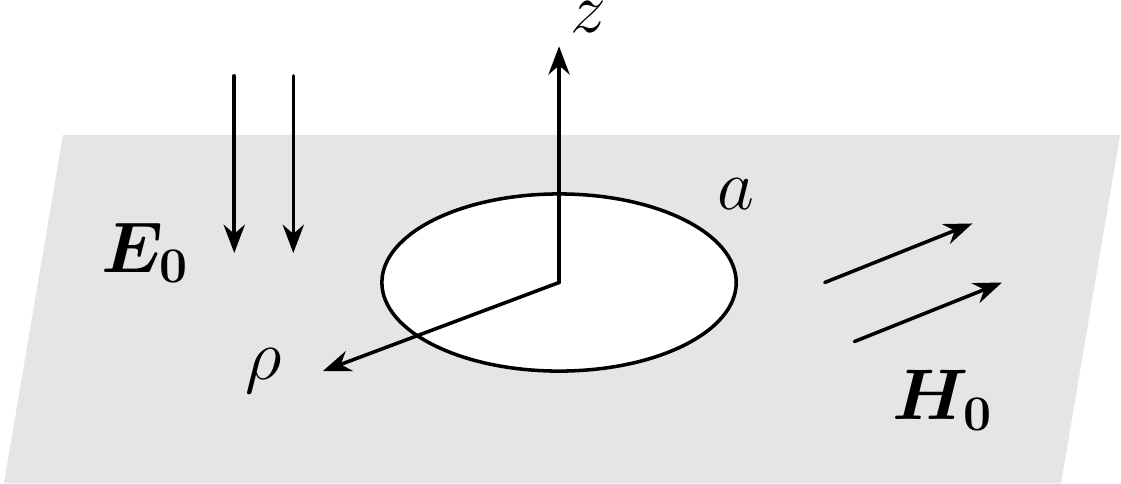
\includegraphics[width=0.4\textwidth]{electrostatics_fig/circular_hole_on_conducting_plane_schematic_diagram.png}
	\caption{导体平面上的圆孔示意图}
	\label{导体平面上的圆孔示意图}
\end{figure}


\subsubsection{电场情况}
若未开孔时，\(z > 0\) 的空间中存在匀强电场 \(\vb{E}_0 = -E_0 \uv{z}\).

记开孔后，导体平面上感应电荷产生的额外电势为 \(\Phi^{(1)}(\rho, z)\)（显然与 \(\phi\) 无关）.易知 \(\Phi^{(1)}(\rho, z) = \Phi^{(1)}(\rho, -z)\)，故空间电势分布为
\begin{equation*}
	\Phi(\rho, z) =
	\begin{cases}
		E_0 z + \Phi^{(1)}(\rho, z), & z > 0, \\
		\Phi^{(1)}(\rho, |z|),       & z < 0.
	\end{cases}
\end{equation*}

圆孔处（\(\rho<a\)）电场连续，得
\begin{equation*}
	\left.\frac{\partial \Phi(\rho, z)}{\partial z}\right|_{z=0^+} = \left.\frac{\partial \Phi(\rho, z)}{\partial z}\right|_{z=0^-} \quad\implies\quad \left.\frac{\partial \Phi^{(1)}(\rho, z)}{\partial z}\right|_{z=0^+} = -\frac{E_0}{2}.
\end{equation*}
考虑到导体接地，故总的边界条件为
\begin{equation*}
	\left.\Phi^{(1)}(\rho, z)\right|_{\rho \ge a,\, z=0} = 0, \quad \left.\frac{\partial \Phi^{(1)}(\rho, z)}{\partial z}\right|_{\rho < a,\, z=0^+} = -\frac{E_0}{2}.
\end{equation*}

除产生 \(\vb{E}_0\) 的源外，导体平面外无电荷，有\(\nabla^2 \Phi^{(1)}(\rho, z) = 0\)，对其做 Hankel 变换
\begin{equation*}
	\Phi^{(1)}(\rho, z) = \int_0^\infty A(k) e^{-k|z|} J_0(k\rho) \,\d k.
\end{equation*}
则边界条件给出
\begin{equation*}
	\int_0^\infty k A(k) J_0(k\rho) \,\d k = \frac{E_0}{2}, \quad \rho < a. \qquad
	\int_0^\infty A(k) J_0(k\rho) \,\d k = 0, \quad \rho \ge a.
\end{equation*}
解得
\begin{equation*}
	&A(k) = \frac{E_0}{\pi} a^2 j_1(ka).\\
	&\Phi^{(1)}(\rho, z)
	= \frac{E_0}{\pi} a^2 \int_0^\infty e^{-k|z|} J_0(k\rho) j_1(ka) \,\d k
	= \frac{E_0}{\pi} a \left( \sqrt{\frac{R-\lambda}{2}} - \frac{|z|}{a} \arctan\sqrt{\frac{2}{R+\lambda}} \right).
\end{equation*}
式中
\begin{equation*}
	\lambda = \frac{z^2 + \rho^2 - a^2}{a^2}, \quad
	R = \sqrt{\lambda^2 + \frac{4z^2}{a^2}}.
\end{equation*}

在一些特殊值及极限位置处
\begin{equation*}
	&\Phi^{(1)}(\rho, z) = E_0
	\begin{cases}
		\dfrac{a}{\pi} \left( 1 - \dfrac{|z|}{a} \arctan\dfrac{a}{|z|} \right),   & \rho = 0,                \\[8pt]
		\dfrac{1}{\pi} \sqrt{a^2 - \rho^2} + \mathcal{O}(z^2),                    & |z| \to 0, \rho \le a,   \\[8pt]
		\left( \dfrac{a}{\sqrt{\rho^2-a^2}} - \arcsin\dfrac{a}{\rho} \right) |z|, & |z| \to 0, \rho > a,     \\[8pt]
		\dfrac{a^3 |z|}{3\pi (\rho^2+z^2)^{3/2}},                                 & \sqrt{\rho^2+z^2} \gg a.
	\end{cases}\\
	&\vb{E}(\rho, z) = -\nabla\Phi(\rho, z) = E_0
	\begin{cases}
		\dfrac{\rho}{\pi\sqrt{a^2-\rho^2}} \uv{\rho} - \Theta(z) \uv{z},                                                       & |z| \to 0, \rho \le a, \\[8pt]
		\left( -\dfrac{a}{\sqrt{\rho^2-a^2}} + \arcsin\dfrac{a}{\rho} \right) \operatorname{sgn}(z) \uv{z} - \Theta(z) \uv{z}, & |z| \to 0, \rho > a,
	\end{cases}
\end{equation*}
其中 \(\Theta(x)\) 是阶跃函数，\(\operatorname{sgn}(z)\) 是符号函数.

可见，在远处（\(\sqrt{\rho^2+z^2} \gg a\)），圆孔的电场作用近似为放在原点的电偶极矩
\begin{equation*}
	\vb{p}_{\text{hole}} = \operatorname{sgn}(z) \frac{4\varepsilon_0}{3} a^3 E_0 \uv{z}.
\end{equation*}
其正负号取决于观测点\(z\)坐标的正负.

\subsubsection{磁场情况}
若未开孔时，\(z > 0\) 的空间中存在匀强磁场 \(\vb{H}_0 = H_0 \uv{y}\).

记开孔后，导体平面上感应电流产生的额外磁势为 \(\Phi_M^{(1)}(\rho, \phi, z)\)（其梯度为磁场强度）.易知 \(\Phi_M^{(1)}(\rho, \phi, z) = -\Phi_M^{(1)}(\rho, \phi, -z)\)，故空间磁势分布为
\begin{equation*}
	\Phi_M(\rho, \phi, z) =
	\begin{cases}
		-H_0 \rho \sin\phi + \Phi_M^{(1)}(\rho, \phi, z), & z > 0, \\[4pt]
		-\Phi_M^{(1)}(\rho, \phi, |z|),                   & z < 0.
	\end{cases}
\end{equation*}

圆孔处磁势连续，\(\left.\Phi_M(\rho, \phi, z)\right|_{z=0^+} = \left.\Phi_M(\rho, \phi, z)\right|_{z=0^-}\)，且导体平面表面无法向磁场，得边界条件为
\begin{equation*}
	\left.\Phi_M^{(1)}(\rho, \phi, z)\right|_{\rho < a,\, z=0} = \frac{H_0}{2} \rho \sin\phi, \qquad
	\left.\frac{\partial \Phi_M^{(1)}(\rho, \phi, z)}{\partial z}\right|_{\rho \ge a,\, z=0^+} = 0.
\end{equation*}

考虑到导体平面外无电流（除产生 \(\vb{H}_0\) 的源外）、无磁化强度，有\(\nabla^2 \Phi_M^{(1)}(\rho, \phi, z) = 0\)，对其做 Hankel 变换
\begin{equation*}
	\Phi_M^{(1)}(\rho, \phi, z) = \int_0^\infty A(k) e^{-k|z|} J_1(k\rho) \sin\phi \,\d k.
\end{equation*}
则边界条件给出
\begin{equation*}
	\int_0^\infty A(k) J_1(k\rho) \,\d k = \frac{H_0}{2} \rho, \quad \rho < a. \qquad
	\int_0^\infty k A(k) J_1(k\rho) \,\d k = 0, \quad \rho \ge a.
\end{equation*}
解得
\begin{align*}
	A(k) & = \frac{2H_0}{\pi} a^2 j_1(ka).                                                                                                                                                         \\
	\Phi_M^{(1)}(\rho, \phi, z)
	     & = \frac{2H_0}{\pi} a^2 \sin\phi \int_0^\infty e^{-k|z|} J_1(k\rho) j_1(ka) \,\d k                                                                                                       \\
	     & = \frac{H_0}{\pi} a \left( \frac{|z|}{\rho} \sqrt{\frac{R-\lambda}{2}} - \frac{a}{\rho} \sqrt{\frac{R+\lambda}{2}} + \frac{\rho}{a} \arctan\sqrt{\frac{2}{R+\lambda}} \right) \sin\phi,
\end{align*}
式中 \(\lambda, R\) 定义同上.

在一些特殊值及极限位置处
\begin{equation*}
	&\Phi_M^{(1)}(\rho, \phi, z) = H_0 \sin\phi
	\begin{cases}
		\left( \dfrac{\rho}{2} - \dfrac{2\rho}{\pi\sqrt{a^2-\rho^2}} \right) |z|,                                       & |z| \to 0, \rho \le a,   \\[8pt]
		\dfrac{\rho}{\pi} \arctan\dfrac{a}{\sqrt{\rho^2-a^2}} - \dfrac{a\sqrt{\rho^2-a^2}}{\pi\rho} + \mathcal{O}(z^2), & |z| \to 0, \rho > a,     \\[8pt]
		\dfrac{2a^3 \rho}{3\pi (\rho^2+z^2)^{3/2}},                                                                     & \sqrt{\rho^2+z^2} \gg a.
	\end{cases}\\
	&\vb{H}(\rho, \phi, z) = -\nabla\Phi_M(\rho, \phi, z) = H_0
	\begin{cases}
		\dfrac12 (\sin\phi \uv{\rho} + \cos\phi \uv{\phi}) + \dfrac{2\rho}{\pi\sqrt{a^2-\rho^2}} \sin\phi \uv{z},                     & |z| \to 0, \rho \le a, \\[8pt]
		-\dfrac{\sin\phi}{\pi} \left( \arctan\dfrac{a}{\sqrt{\rho^2-a^2}} - \dfrac{a(a^2+\rho^2)}{\pi\rho^2\sqrt{\rho^2-a^2}} \right) \uv{\rho}                \\[6pt]
		\quad -\dfrac{\cos\phi}{\pi} \left( \arctan\dfrac{a}{\sqrt{\rho^2-a^2}} - \dfrac{a\sqrt{\rho^2-a^2}}{\rho} \right) \uv{\phi}, & |z| \to 0, \rho > a.
	\end{cases}
\end{equation*}

可见，在远处（\(\sqrt{\rho^2+z^2} \gg a\)），圆孔的磁场作用近似为放在原点的磁偶极矩
\begin{equation*}
	\vb{m}_{\text{hole}} = \operatorname{sgn}(z) \frac{8}{3} a^3 H_0 \uv{y}.
\end{equation*}
其正负号亦取决于观测点\(z\)坐标的正负.

\subsection{旋转对称荷流分布的电磁场}
在球坐标系下，若 \(\vb{J}(\vb{r}) = J(r,\theta) \uv{\phi} = J(r,\theta) (-\sin\phi \uv{x} + \cos\phi \uv{y})\)，则 \(A_z = 0\)，
\begin{equation*}
	\tilde{A}(\vb{r}) = A_y + iA_x
	= \frac{\mu_0}{4\pi} \int \frac{\vb{J}(\vb{r}') \cdot (\uv{y}' + i\uv{x}')}{|\vb{r} - \vb{r}'|} \,\d \vb{r}'
	= \frac{\mu_0}{4\pi} \int \frac{J(r',\theta') e^{-i\phi}}{|\vb{r} - \vb{r}'|} \,\d \vb{r}'.
\end{equation*}
运用数学公式
\begin{equation*}
	\frac{1}{|\vb{r} - \vb{r}'|} = \sum_{l=0}^\infty \sum_{m=-l}^l \frac{4\pi}{2l+1} \frac{r_<^l}{r_>^{l+1}} Y_{lm}^*(\theta',\phi') Y_{lm}(\theta,\phi),\quad r_< = \min\{r, r'\},\quad r_> = \max\{r, r'\}
\end{equation*}
得
\begin{align*}
	\tilde{A}(\vb{r})
	               & = \frac{\mu_0}{2} e^{-i\phi} \sum_{l=1}^\infty P_l^1(\cos\theta) \frac{1}{l(l+1)} \iint \frac{r_<^l}{r_>^{l+1}} J(r',\theta') P_l^1(\cos\theta') (r')^2 \sin\theta' \,\d \theta' \d r', \\[4pt]
	\vb{A}(\vb{r})
	               & = A_\phi \uv{\phi} = (\cos\phi \operatorname{Re}\tilde{A} - \sin\phi \operatorname{Im}\tilde{A}) \uv{\phi}
	= \frac{\mu_0}{2}\uv{\phi} \sum_{l=1}^\infty P_l^1(\cos\theta) \frac{1}{l(l+1)} \iint \frac{r_<^l}{r_>^{l+1}} J(r',\theta') P_l^1(\cos\theta') (r')^2 \sin\theta' \,\d \theta' \d r' .                   \\
	\vb{B}(\vb{r}) & = \nabla \times \vb{A}
	= \frac{1}{r\sin\theta} \frac{\partial (\sin\theta A_\phi)}{\partial \theta} \uv{r} - \frac{1}{r} \frac{\partial (r A_\phi)}{\partial r} \uv{\theta}
	\\&= -\frac{\mu_0}{2r} \sum_{l=1}^\infty \left( \uv{r} P_l(\cos\theta) + \uv{\theta} \frac{P_l^1(\cos\theta)}{l(l+1)} \frac{\partial}{\partial r} r \right) \iint \frac{r_<^l}{r_>^{l+1}} J(r',\theta') P_l^1(\cos\theta') (r')^2 \sin\theta' \,\d \theta' \d r'.
\end{align*}

同理，在球坐标系下，若 \(\rho(\vb{r}) = \rho(r,\theta)\)，则
\begin{align*}
	\Phi(\vb{r})
	 & = \frac{1}{4\pi\varepsilon_0} \int \frac{\rho(\vb{r}')}{|\vb{r} - \vb{r}'|} \,\d \vb{r}' = \frac{1}{2\varepsilon_0} \sum_{l=0}^\infty P_l(\cos\theta) \iint \frac{r_<^l}{r_>^{l+1}} \rho(r',\theta') P_l(\cos\theta') (r')^2 \sin\theta' \,\d \theta' \d r',                   \\[4pt]
	\vb{E}(\vb{r})
	 & = -\nabla\Phi = -\frac{1}{2\varepsilon_0} \sum_{l=0}^\infty \left( \frac{\uv{\theta}}{r} P_l^1(\cos\theta) + \uv{r} P_l(\cos\theta) \frac{\partial}{\partial r} \right) \iint \frac{r_<^l}{r_>^{l+1}} \rho(r',\theta') P_l(\cos\theta') (r')^2 \sin\theta' \,\d \theta' \d r'.
\end{align*}

\subsection{磁场扩散问题}
在电导率为 \(\sigma\)、磁导率为 \(\mu\) 的良导体 (\(\sigma\tau \gg \varepsilon\)，\(\tau\) 为外场特征变化时间，\(\varepsilon\) 为导体介电常数) 中，麦克斯韦方程组简化为：
\begin{equation*}
	\nabla \times \vb{B} \approx \mu \vb{J}, \quad
	\nabla \cdot \vb{B} = 0, \quad
	\nabla \times \vb{E} + \frac{\partial \vb{B}}{\partial t} = 0, \quad
	\nabla \cdot \vb{E} = 0, \quad
	\vb{J} = \sigma \vb{E}.
\end{equation*}
得
\begin{equation*}
	\bigl(\nabla^2 - \mu\sigma \frac{\partial}{\partial t}\bigr) \vb{f}(\vb{r}, t) = 0, \qquad
	\vb{f} = \vb{B} \;\text{or } \vb{E} \;\text{or } \vb{J} \;\text{ or } \vb{A}\;(\vb{B} = \nabla \times \vb{A}).
\end{equation*}
依据该矢量扩散方程，可以求出良导体内电磁场突变时，其达到稳态前的扩散特性.

\subsubsection{球坐标系下的解}
标量扩散方程 \((\nabla^2 - \mu\sigma \partial/\partial t) g(\vb{r}, t) = 0\) 在球坐标下的形式解为：
\begin{equation*}
	g(\vb{r}, t) &= \int_0^\infty \sum_{l=0}^\infty \sum_{m=-l}^l e^{-k^2 t/(\mu\sigma)} a_{lm}(k) j_l(kr) Y_{lm}(\theta,\phi) \,\d k,\\
	a_{lm}(k) &= \frac{2k^2}{\pi} \int_0^{2\pi} \int_0^\pi \int_0^\infty g(\vb{r}, t=0) j_l(kr) Y_{lm}^*(\theta,\phi) r^2 \sin\theta \,\d r \,\d \theta \,\d \phi.
\end{equation*}

特别地，若 \(g(\vb{r}, t) = a(r, t=0) \,b(\theta,\phi)\)，则
\begin{equation*}
	g(\vb{r}, t) = a(r,t)\, b(\theta,\phi),\quad
	a(r,t) = \sum_{l=0}^\infty \int_0^\infty \int_0^\infty \frac{2k^2}{\pi} r'^2 j_l(kr') a(r',t=0) e^{-k^2 t/(\mu\sigma)} j_l(kr) \,\d r' \,\d k.
\end{equation*}

特别地，若 \(\vb{f}(\vb{r}, t=0) = f_\phi(r, t=0) \sin\theta \uv{\phi}\)，即其在直角坐标系下可写作
\begin{equation*}
	\vb{f}(\vb{r}, t=0) = f_\phi(r, t=0) \sqrt{\frac{2\pi}{3}} \bigl[-i(Y_{1,-1} - Y_{1,1}) \uv{x} - (Y_{1,-1} + Y_{1,1}) \uv{y}\bigr],
\end{equation*}
则分离变量法给出
\begin{equation*}
	\vb{f}(\vb{r}, t) = f_\phi(r,t) \sin\theta\, \uv{\phi},\qquad
	f_\phi(r,t) = \int_0^\infty \int_0^\infty \frac{2k^2}{\pi} r'^2 j_1(kr') f_\phi(r',t=0) e^{-k^2 t/(\mu\sigma)} j_1(kr) \,\d r' \,\d k.
\end{equation*}

\begin{notes}
	用格林函数的方法，也可以写出球坐标系下积分形式的解.
	扩散方程在三维无界空间的格林函数满足
	\begin{equation*}
		\bigl(\nabla^2 - \mu\sigma \frac{\partial}{\partial t}\bigr) G(\vb{r},\vb{r}',t) = \delta(\vb{r} - \vb{r}') \Theta(t),
	\end{equation*}
	解得
	\begin{equation*}
		G(\vb{r},\vb{r}',t) = G(\vb{r} - \vb{r}',t)
		= \frac{\Theta(t)}{(2\pi)^3} \int e^{-k^2 t/(\mu\sigma)} e^{i\vb{k}\cdot(\vb{r} - \vb{r}')} \,\d \vb{k}
		= \Theta(t) \left(\frac{\mu\sigma}{4\pi t}\right)^{3/2} e^{-\mu\sigma |\vb{r} - \vb{r}'|^2/(4t)}.
	\end{equation*}
	进而，扩散方程的解为
	\begin{equation*}
		\vb{A}(\vb{r},t) = \int G(\vb{r} - \vb{r}',t) \vb{A}(\vb{r}',t=0) \,\d \vb{r}'
		= \int \left(\frac{\mu\sigma}{4\pi t}\right)^{3/2} e^{-\mu\sigma |\vb{r} - \vb{r}'|^2/(4t)} \vb{A}(\vb{r}',t=0) \,\d \vb{r}'.
	\end{equation*}
\end{notes}

\subsubsection{磁场扩散实例}

\begin{example}
	电导率为 \(\sigma\)、磁导率为 \(\mu\) 的良导体液中，半径为 \(a\) 的球面上固定有导线，在球面内产生 \(B_0 \uv{z}\) 的匀强磁场，在球面外产生等效磁偶极矩为 \(4\pi a^3 B_0 \uv{z}/\mu\) 的偶极矩磁场.在 \(t=0\) 时刻突然切断导线的电流，使空间中无电流分布，此后磁场将扩散.

	易知，电流密度、磁矢势为
	\begin{equation*}
		\vb{J}(\vb{r}, t=0) = \frac{3B_0}{2\mu} \delta(r-a) \sin\theta \uv{\phi},\quad
		\vb{A}(\vb{r}, t=0)= A_\phi(r,t=0) \sin\theta \uv{\phi},\quad
		A_\phi(r,t=0) = \frac{B_0 a^2}{2} \frac{r_<}{r_>^2},
	\end{equation*}
	其中 \(r_< = \min\{r,a\}\), \(r_> = \max\{r,a\}\).

	用分离变量法解得
	\begin{align*}
		A_\phi(r,t) & = \int_0^\infty \int_0^\infty \frac{2k^2}{\pi} r'^2 j_1(kr') \frac{B_0 a^2}{2} \frac{r'_<}{(r'_>)^2} e^{-k^2 t/(\mu\sigma)} j_1(kr) \,\d r' \,\d k                                             \\
		            & = \frac{3B_0 a^2}{\pi} \int_0^\infty j_1(kr) j_1(ka) e^{-k^2 t/(\mu\sigma)} \,\d k                                                                                                             \\
		            & = \frac{B_0 r}{12\sqrt{\pi} (\nu t)^{3/2}} \sum_{m=0}^\infty \frac{3(-1)^m}{2^{2m} m! (3+2m)} \left(\frac{r^2}{a^2 \nu t}\right)^m \,_2F\left(-m, -m-\frac32; \frac52; \frac{a^2}{r^2}\right),
	\end{align*}
	式中\(\nu = (\mu\sigma a^2)^{-1}\)，\(_2F(\alpha,\beta.\gamma.z)\) 为超几何函数
	\begin{equation*}
		_2F\!\left(-m, -m-\frac32; \frac52; \frac{a^2}{r^2}\right) = \sum_{n=0}^m \frac{12(2m+3)(m-n+1)(n+1)(2m+1)!}{(2m-2n+3)! (2n+3)!} \left(\frac{a^2}{r^2}\right)^{m-n}.
	\end{equation*}
	因此
	\begin{equation*}
		A_\phi(r,t) = \frac{B_0 r}{2} \sum_{m=0}^\infty \sum_{n=0}^m \frac{3(-1)^m (m-n+1)(n+1)(2m+1)!}{\sqrt{\pi}\,2^{2m-1} m! (2m-2n+3)! (2n+3)!} (\nu t)^{-m-3/2} \left(\frac{r^2}{a^2}\right)^n.
	\end{equation*}

	进而，磁场在柱坐标下的分量可以求出为
	\begin{align*}
		\vb{B}(\vb{r},t) = \nabla \times \vb{A}(\vb{r},t)
		= \left[\frac{2A_\phi}{r} \cos^2\theta + \frac{1}{r} \frac{\partial(rA_\phi)}{\partial r} \sin^2\theta\right] \uv{z}
		+ \left[\frac{2A_\phi}{r} - \frac{1}{r} \frac{\partial(rA_\phi)}{\partial r}\right] \sin\theta \cos\theta \uv{\rho},
	\end{align*}
	式中 \(\uv{z} = \uv{r}\cos\theta - \uv{\theta}\sin\theta\), \(\uv{\rho} = \uv{r}\sin\theta + \uv{\theta}\cos\theta\).

	在 \(r \ll a\) 处，最低阶为 \(n=0\) 项（球心磁场演化图像如图\ref{球域磁场扩散示意图}）
	\begin{align*}
		 & A_\phi(r \ll a, t) = \frac{B_0 r}{2} \sum_{m=0}^\infty \frac{(-1)^m}{\sqrt{\pi}\,2^{2m+1} m! (2m+3)} (\nu t)^{-m-3/2}
		= \frac{B_0 r}{2} \left[ \operatorname{erf}\!\left(\frac{1}{2\sqrt{\nu t}}\right) - \frac{1}{\sqrt{\pi\nu t}} e^{-1/(4\nu t)} \right],                   \\
		 & \vb{B}(\vb{r}=0, t) = B_0 \uv{z} \left[ \operatorname{erf}\!\left(\frac{1}{2\sqrt{\nu t}}\right) - \frac{1}{\sqrt{\pi\nu t}} e^{-1/(4\nu t)} \right], \\
		 & A_\phi(r, t \gg 1/\nu) = \frac{B_0 r}{12\sqrt{\pi}} (\nu t)^{-3/2}.\quad
		\vb{B}(r, t \gg 1/\nu) = \frac{B_0}{6\sqrt{\pi}} (\nu t)^{-3/2} \uv{z}.
	\end{align*}

	另外，由于电流密度也满足扩散方程，且其形式为
	\begin{equation*}
		\vb{J}(\vb{r}, t=0) = J_\phi(r, t=0) \sin\theta \uv{\phi},\quad J_\phi(r, t=0) = \frac{3B_0}{2\mu} \delta(r-a)
	\end{equation*}
	进而
	\begin{align*}
		J_\phi(r,t) & = \int_0^\infty \int_0^\infty \frac{2k^2}{\pi} r'^2 j_1(kr') \frac{3B_0}{2\mu} \delta(r'-a) e^{-k^2 t/(\mu\sigma)} j_1(kr) \,\d r' \,\d k                                                     \\
		            & = \frac{3B_0 a^2}{\pi\mu} \int_0^\infty k^2 j_1(ka) j_1(kr) e^{-k^2 t/(\mu\sigma)} \,\d k                                                                                                     \\
		            & = \frac{B_0 r}{\sqrt{\pi}\mu a^2 (\nu t)^{5/2}} \sum_{m=0}^\infty \frac{(-1)^m}{2^{2m+3} m!} \left(\frac{r^2}{a^2 \nu t}\right)^m _2F\!\left(-m, -m-\frac32. \frac52. \frac{a^2}{r^2}\right).
	\end{align*}
	或将其展开为
	\begin{equation*}
		&J_\phi(r,t) = \frac{B_0 r}{8\sqrt{\pi}\mu a^2} \sum_{m=0}^\infty \sum_{n=0}^m \frac{3(-1)^m (2m+3)(2m+1)!}{2^{2m} m! (2n+3)(2m-2n+3)(2m-2n+1)! (2n+1)! (\nu t)^{m+5/2}} \left(\frac{r^2}{a^2}\right)^n.\\
		&J_\phi(r \ll a, t) = \frac{B_0 r}{8\sqrt{\pi}\mu a^2} (\nu t)^{-5/2} e^{-1/(4\nu t)}, \quad
		J_\phi(r, t \gg 1/\nu) = \frac{B_0 r}{8\sqrt{\pi}\mu a^2} (\nu t)^{-5/2}.
	\end{equation*}

	进而，空间中电磁场的总能量为：
	\begin{align*}
		W_m(t) & = \frac12 \int \vb{J}(\vb{r},t) \cdot \vb{A}(\vb{r},t) \,\d \vb{r}
		= \frac{4\pi}{3} \int_0^\infty J_\phi(r,t) A_\phi(r,t) \,\d r                                                                                                            \\
		       & = \frac{B_0^2 a^3 \sqrt{2\pi}}{24 (\nu t)^{3/2}} \sum_{m=0}^\infty \frac{3(-1)^m}{2^{3m} m! (3+2m)} (\nu t)^{-m}\, _2F\!\left(-m, -m-\frac32. \frac52. 1\right) \\
		       & = \frac{B_0^2 a^3 \sqrt{2\pi}}{24 (\nu t)^{3/2}} \sum_{m=0}^\infty \frac{9(-1)^m (m+1)}{2^{m-1} (m+3)! (2m+3)} (\nu t)^{-m},                                    \\
		W_m(t  & \gg 1/\nu) = \frac{B_0^2 a^3 \sqrt{2\pi}}{24 (\nu t)^{3/2}}.
	\end{align*}
\end{example}

\begin{example}
	在电导率为 \(\sigma\)、磁导率为 \(\mu\) 的空间中，于 \(z = \pm a\) 平面上，有电流密度
	\begin{equation*}
		\vb{J}(\vb{r}, t=0) = H_0 \bigl[\delta(z+a) - \delta(z-a)\bigr] \uv{y},
	\end{equation*}
	这将使得空间中存在磁场强度
	\begin{equation*}
		\vb{H}(\vb{r}, t=0) = H_0 \bigl[\Theta(z+a) - \Theta(z-a)\bigr] \uv{x},
	\end{equation*}
	\(t=0\) 时刻关闭电源，停止电流输入，求空间中磁场的扩散.

	易知，\(\vb{H}(\vb{r}, t) = H(z,t) \uv{x}\)，磁场矢量的扩散退化为 \(\uv{x}\) 方向分量的标量扩散.采用拉普拉斯变换，记 \(\tilde{H}(z,p) = \mathcal{L}^{-1}\{H(z,t)\}(p)\)，代入扩散方程得
	\begin{equation*}
		\bigl(\nabla^2 - \mu\sigma \frac{\partial}{\partial t}\bigr) \vb{H}(\vb{r},t) = 0\quad\implies\quad \left(\frac{\partial^2}{\partial z^2} + \mu\sigma p\right) \tilde{H}(z,p) = 0.
	\end{equation*}
	显然，\(\tilde{H}(z,p) = \tilde{H}(-z,p)\)，记 \(k^2 = \mu\sigma p\)，解得
	\begin{equation*}
		\tilde{H}(z,p) = h(k) \cos(kz), \quad
		\vb{H}(\vb{r},t) = \mathcal{L}\{\tilde{H}(z,p)\}(t) \uv{x} = \uv{x} \int_0^\infty h(k) \cos(kz) e^{-k^2 t/(\mu\sigma)} \,\d k.
	\end{equation*}
	代入初始条件得
	\begin{equation*}
		h(k) = \frac{1}{\pi} \int_{-\infty}^\infty H(z,t=0) \cos(kz) \,\d z = \frac{2H_0}{\pi k} \sin(ka).
	\end{equation*}
	进而（演化图像如图\ref{一维磁场扩散示意图}）
	\begin{align*}
		\vb{H}(\vb{r},t) & = \uv{x} \int_0^\infty h(k) \cos(kz) e^{-k^2 t/(\mu\sigma)} \,\d k
		= \frac{H_0}{2} \uv{x} \left[ \operatorname{erf}\!\left(\frac{1 + |z|/a}{2\sqrt{\nu t}}\right) + \operatorname{erf}\!\left(\frac{1 - |z|/a}{2\sqrt{\nu t}}\right) \right],          \\
		\vb{H}(\vb{r}, t & \gg 1/\nu) = \frac{H_0}{\sqrt{\pi\nu t}} e^{-z^2/(4\nu t a^2)} \left(1 - \frac{1}{12\nu t} + \frac{z^2}{24\nu^2 t^2 a^2} + \frac{1}{160\nu^2 t^2}\right) \uv{x}.
	\end{align*}

	\begin{figure}[H]
		\centering
		\begin{minipage}[b]{0.49\textwidth}
			\centering
			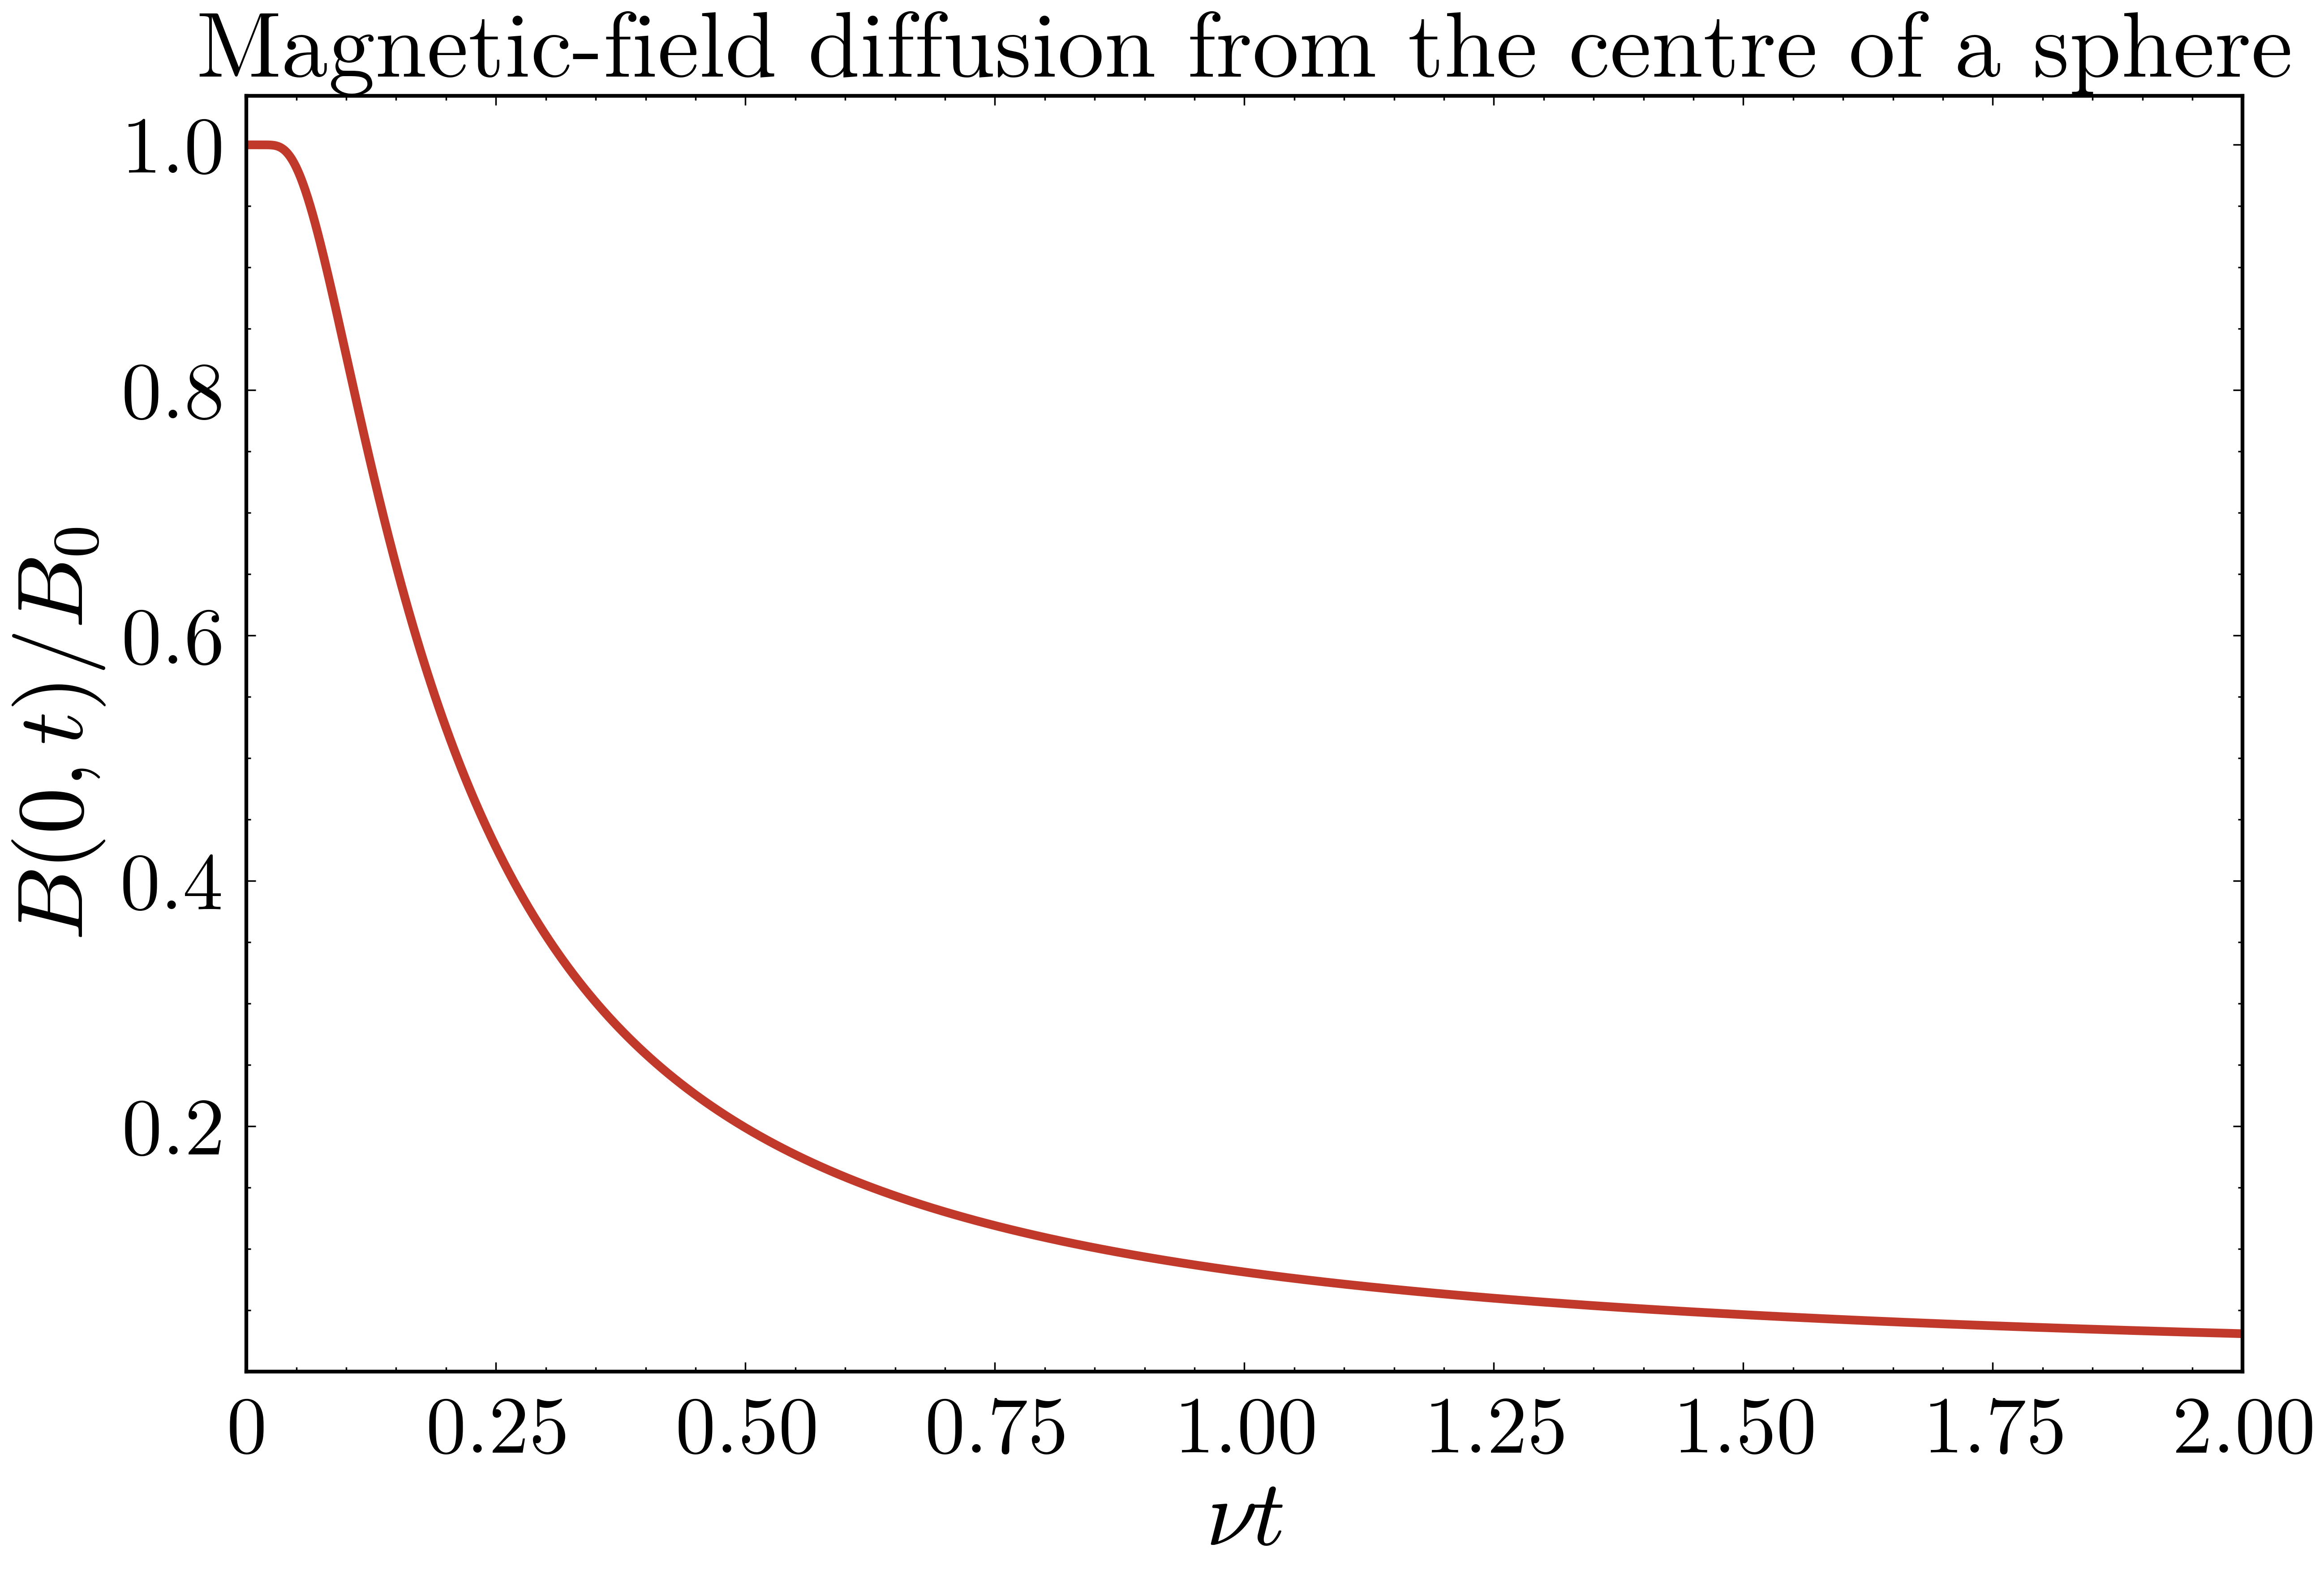
\includegraphics[width=\textwidth]{electrostatics_fig/magnetic_field_diffusion_from_sphere_center_schematic_diagram.png}
			\caption{球心磁场扩散示意图}
			\label{球心磁场扩散示意图}
		\end{minipage}
		\hfill
		\begin{minipage}[b]{0.49\textwidth}
			\centering
			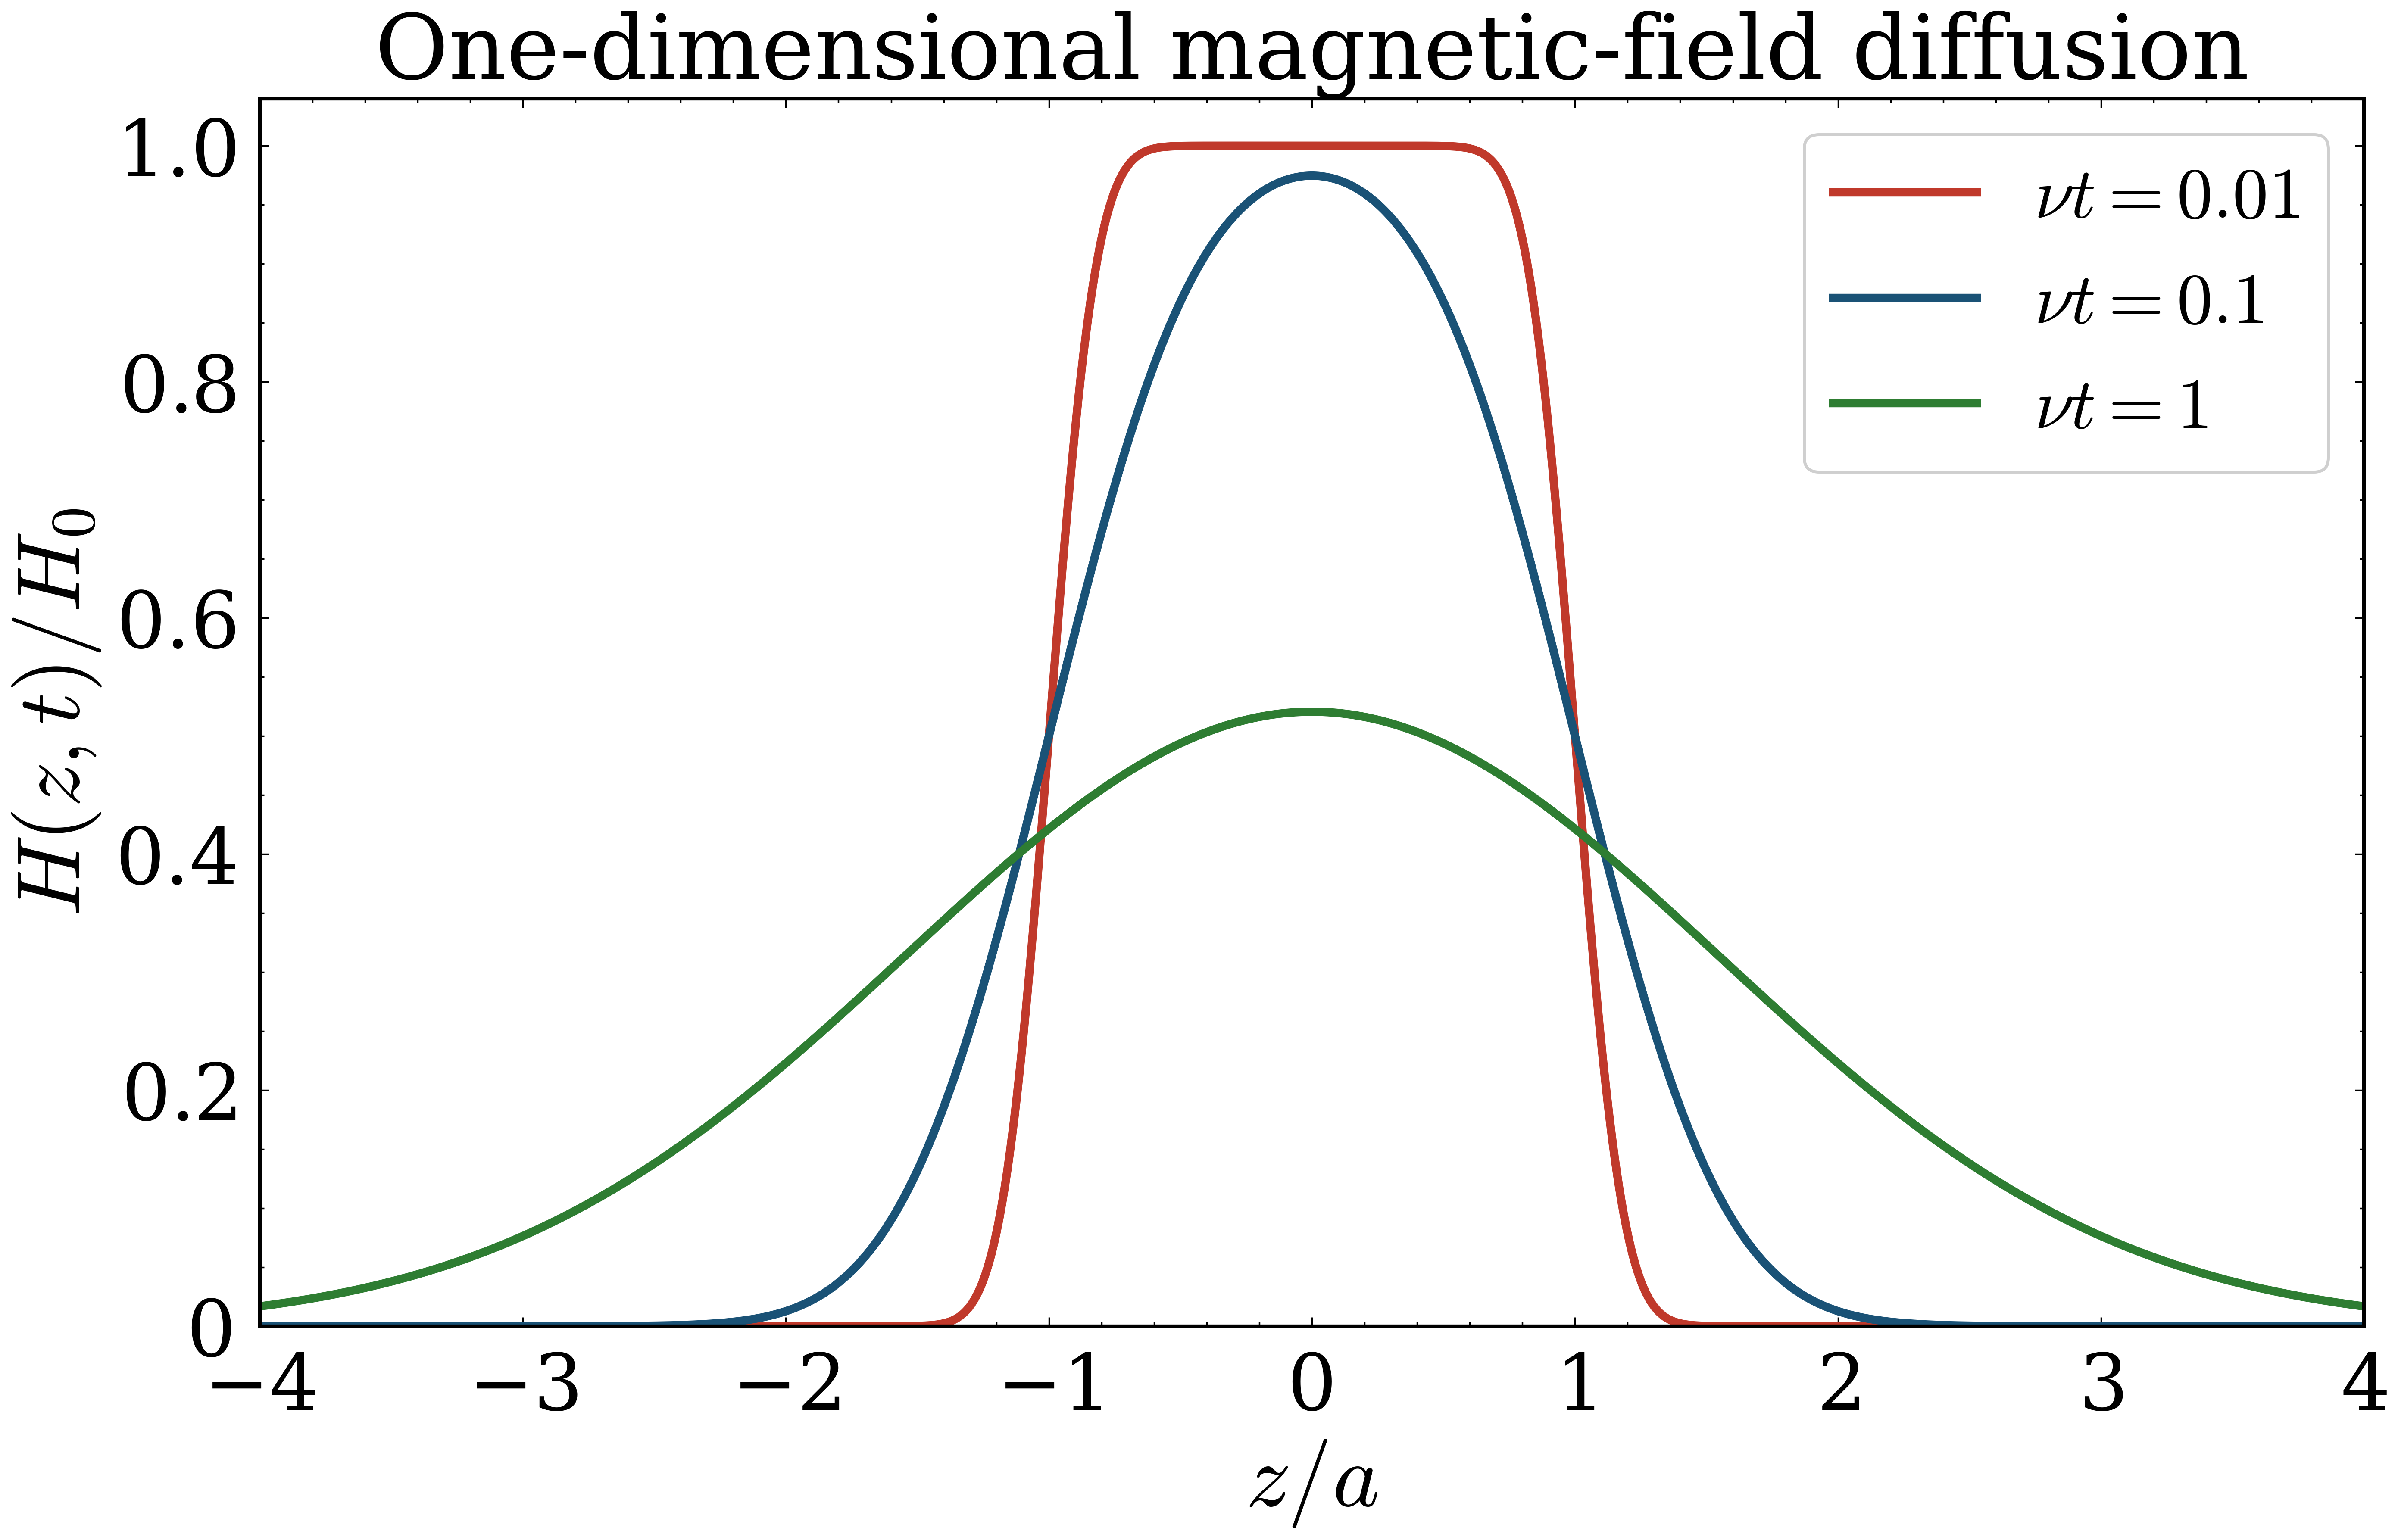
\includegraphics[width=\textwidth]{electrostatics_fig/one_dimensional_magnetic_field_diffusion_schematic_diagram.png}
			\caption{一维磁场扩散示意图}
			\label{一维磁场扩散示意图}
		\end{minipage}
	\end{figure}
\end{example}
